\documentclass[11pt]{article}

\usepackage[a4paper,margin=2.5cm]{geometry}
\usepackage{fontspec}
\setmainfont{Latin Modern Roman}
\usepackage{booktabs}
\usepackage{longtable}
\usepackage{array}
\usepackage[table]{xcolor}
\usepackage{listings}
\usepackage{hyperref}
\usepackage{parskip}
\usepackage{amsmath}
\usepackage{microtype}
\usepackage{enumitem}
\usepackage{tikz}
\usepackage{graphicx}
\usetikzlibrary{arrows.meta,positioning,calc,fit,backgrounds,decorations.pathreplacing}

\hypersetup{
  colorlinks=true,
  linkcolor=blue!50!black,
  citecolor=blue!50!black,
  urlcolor=blue!50!black
}

\lstset{
  basicstyle=\ttfamily\footnotesize,
  breaklines=true,
  columns=fullflexible,
  keepspaces=true,
  frame=single,
  backgroundcolor=\color{gray!5},
  captionpos=b
}

\newcommand{\code}[1]{\texttt{#1}}
\newcommand{\class}[1]{\texttt{#1}}
\newcommand{\gain}[1]{\textbf{#1}}

\title{Transactional Support via OSIC on the cMVBT: \\
  System Design, Datastructure Changes, and Optimizations}
\author{Amir Tonta}
\date{August 2026}

\begin{document}
\maketitle

\begin{abstract}
This document describes the cMVBT-OSIC system from first principles: what it is, what it supports,
and how every change to the underlying multiversion B-tree datastructure and every optimization was
measured. The system provides Transactional Support with Snapshot Isolation and Ordered Snapshot
Instant Commit (OSIC) semantics on top of a cache-friendly multiversion B-tree. The document
progresses systematically from foundational concepts through datastructure modifications, then
catalogs optimizations organized by their problem statement, proposed solutions, measured
performance impact, and final adoption decision. Each optimization includes concrete performance
numbers where available, or describes the isolated tests used to measure them.
\end{abstract}

\tableofcontents

\newpage

\section{System Overview}
\label{sec:overview}

\subsection{Purpose and Capabilities}

The cMVBT-OSIC system implements a high-performance, in-memory multiversion B-tree supporting
snapshot isolation transactions. Its primary design goal is to achieve competitive transaction
throughput while maintaining cache efficiency across both transactional (OLTP) and analytical
(OLAP) workloads.

\subsubsection{Transactional Model}

The system provides two transaction modes:

\begin{itemize}
  \item \textbf{Real Transactions:} Multi-statement, snapshot-isolated transactions with
        explicit begin/commit semantics. A transaction registers a single snapshot at its
        start and maintains that snapshot throughout its lifetime.

  \item \textbf{Atomic Operations:} Single-key, auto-committed operations (point reads,
        inserts, updates, deletes) that use the newest committed state rather than a
        registered snapshot.
\end{itemize}

Real transactions follow a First-Writer-Wins conflict resolution policy: when two transactions
attempt to write the same key, the first to reach the leaf successfully applies its change;
the second encounters a conflict and must retry or abort.

\subsubsection{Concurrency Control}

The system combines:

\begin{itemize}
  \item \textbf{Optimistic Lock Coupling (OLC):} Readers sample each node's version number,
        inspect immutable content, validate the version before relying on results, and retry
        if a writer changed the node.

  \item \textbf{Ordered Snapshot Instant Commit (OSIC):} Visibility is determined by a global
        logical clock. Every transaction and atomic operation receives a \code{ts\_start}
        timestamp for reading, and committed changes append to a per-worker commit log indexed
        by timestamp. A reader is visible to a transaction if its commit timestamp falls within
        the transaction's snapshot window.
\end{itemize}

Writers acquire exclusive node guards only for mutation. Readers take no locks.

\subsubsection{Garbage Collection}

The system tracks the oldest active snapshot (either registered in a real transaction or pinned
during a traversal). Version chains and retired blocks are reclaimed only after all snapshots
that could observe them have completed. A sharded, lock-free reuse pool returns retired blocks
to allocators when safe to do so.

\subsubsection{Durability}

Write-Ahead Logging (WAL) is optional and configurable. In-memory mode disables WAL entirely;
durable configurations offer either sharded group-commit channels or lock-free per-thread
batched writes with atomic offset reservation.

\subsection{Architectural Layers}

The system is built in layers, each depending on the ones beneath it:

\begin{enumerate}
  \item \textbf{Physical Page Layout:} Dense key arrays, parallel version/payload arrays,
        inline validity masks.

  \item \textbf{Leaf Access Patterns:} Backward-ordered version lookup, split layout
        effectiveness for cache pressure.

  \item \textbf{Node Synchronization:} Optimistic lock coupling with version validation.

  \item \textbf{Structural Maintenance:} Splitting and merging leaves and internal pages
        while preserving snapshot consistency.

  \item \textbf{Transaction State:} Snapshots, write sets, transaction-local mutation.

  \item \textbf{Garbage Collection and Sharding:} Reclaiming pages, partitioning shared
        structures to reduce contention.

  \item \textbf{Visibility Caching:} Per-worker, per-database snapshot caches and commit-log
        position memoization.

  \item \textbf{Write-Ahead Logging:} Decoupling visibility (in-memory, instant) from
        durability (asynchronous or batched to disk).
\end{enumerate}

\newpage

\section{Datastructure Changes}
\label{sec:datastruct}

This section documents each modification made to the cMVBT's core data layout and how each
change supports the transaction semantics described above.

\subsection{Leaf Page Layout}

\subsubsection{Problem}

A straightforward multiversion B-tree stores complete records as an array of structs
(AoS): \code{[Record \{ key, begin\_ts, end\_ts, payload \}; ...]}. During point lookup,
which walks the array backward searching for the newest visible version of a key, every
entry's version metadata must be loaded into the CPU's cache even when the key does not
match, wasting cache bandwidth on unrelated records.

\subsubsection{Solution: Split Layout}

The leaf stores keys in one dense region and metadata in a separate parallel region:

\begin{figure}[h]
\centering
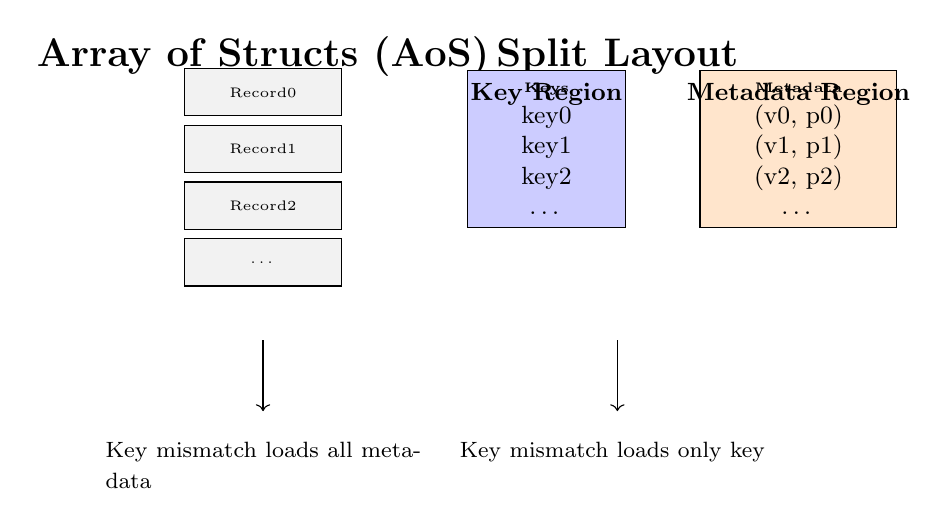
\begin{tikzpicture}[scale=0.9, every node/.style={font=\small}]
  % Array of Structs (AoS) - left side
  \node[font=\Large\bfseries] at (2.5, 5.5) {Array of Structs (AoS)};

  \node[draw, rectangle, fill=gray!10, minimum width=2cm, minimum height=0.6cm, align=center, font=\tiny] (k0) at (2.5, 5) {Record0};
  \node[draw, rectangle, fill=gray!10, minimum width=2cm, minimum height=0.6cm, align=center, font=\tiny] (k1) at (2.5, 4.2) {Record1};
  \node[draw, rectangle, fill=gray!10, minimum width=2cm, minimum height=0.6cm, align=center, font=\tiny] (k2) at (2.5, 3.4) {Record2};
  \node[draw, rectangle, fill=gray!10, minimum width=2cm, minimum height=0.6cm, align=center, font=\tiny] (k3) at (2.5, 2.6) {\ldots};

  \node[right of=k0, xshift=1.2cm, font=\small\color{red}] at (k0.east) {32 bytes};
  \node[right of=k1, xshift=1.2cm, font=\small\color{red}] at (k1.east) {32 bytes};
  \node[right of=k2, xshift=1.2cm, font=\small\color{red}] at (k2.east) {32 bytes};

  % Split Layout - right side
  \node[font=\Large\bfseries] at (7.5, 5.5) {Split Layout};

  % Key region
  \node[draw, rectangle, fill=blue!20, minimum width=2cm, minimum height=2cm, align=center] (keys) at (6.5, 4.2) {
    \tiny \textbf{Keys} \\
    key0 \\ key1 \\ key2 \\ \ldots
  };
  \node[above of=keys, yshift=-0.3cm] {\bfseries Key Region};

  % Metadata region
  \node[draw, rectangle, fill=orange!20, minimum width=2.5cm, minimum height=2cm, align=center, right of=keys, xshift=1.3cm] (meta) at (7.5, 4.2) {
    \tiny \textbf{Metadata} \\
    (v0, p0) \\ (v1, p1) \\ (v2, p2) \\ \ldots
  };
  \node[above of=meta, yshift=-0.3cm] {\bfseries Metadata Region};

  % Arrow showing cache line benefit
  \draw[->] (2.5, 1.5) -- (2.5, 0.5);
  \node[below, text width=4cm] at (2.5, 0.2) {\footnotesize Key mismatch loads all metadata};

  \draw[->] (7.5, 1.5) -- (7.5, 0.5);
  \node[below, text width=4cm] at (7.5, 0.2) {\footnotesize Key mismatch loads only key};
\end{tikzpicture}
\caption{Split layout separates keys from metadata, allowing point lookup to reject unmatched
keys without loading their version/payload cache lines.}
\label{fig:leaf_layout}
\end{figure}

Point lookup first tests the key without loading metadata, reducing cache-line traffic when
keys do not match. Scans can likewise test key ranges before touching metadata cache lines.

\subsubsection{Measured Performance}

An isolated microbenchmark (`tools/leaf_layout_bench.rs`) compared the layouts on a 62.5 MiB
working set of independently boxed leaves:

\begin{table}[h]
\centering
\small
\begin{tabular}{lrrr}
\toprule
\textbf{Operation} & \textbf{AoS (Mlookups/s)} & \textbf{Split (Mlookups/s)} & \textbf{Speedup} \\
\midrule
Point: latest visible & 30.57 & 33.17 & 1.085$\times$ \\
Point: one-version fallback & 18.43 & 20.15 & 1.093$\times$ \\
Point: three-version fallback & 9.03 & 11.02 & 1.221$\times$ \\
Scan: full leaves & 322.84 Mslots/s & 320.65 Mslots/s & 0.993$\times$ \\
Scan: 50\% key ranges & 338.50 & 344.77 & 1.019$\times$ \\
Scan: 20\% key ranges & 354.82 & 389.09 & 1.097$\times$ \\
\bottomrule
\end{tabular}
\caption{Split layout improves point lookup (8.5--22.1\%) and selective scans (1.9--9.7\%),
with full scans unchanged. The multi-leaf working set is more representative of real trees
than a single hot page.}
\label{tab:leaf_layout}
\end{table}

\textbf{Decision:} Adopted. The improvement in lookups with multiple version fallbacks
(which are common on hot keys in contended workloads) and in selective scans outweighs the
zero-cost for full scans.

\subsection{Inline Validity Mask}

\subsubsection{Problem}

A normal leaf has at most 123 physical slots. Recording whether each slot was invalidated
(e.g., by a transaction abort) naively requires either a per-slot atomic or a separate
heap-allocated bitmap, both adding indirection and allocator traffic.

\subsubsection{Solution}

Store validity as two inline \code{AtomicU64} words (128 bits total), directly in the page.
A clear bit means "invalidated"; this is a \emph{physical} validity mask, not an MVCC
visibility mask, which still depends on the querying transaction's snapshot. Lookup can
skip invalidated slots before loading their version headers, avoiding cache misses on
aborted entries.

Oversized leaf variants (used for TPC-C's hot Warehouse and District tables) use a same-sized
union that stores a heap bitmap for larger capacities.

\subsubsection{Measured Performance}

The validity mask is a building block enabling faster lookup; its performance is subsumed
in end-to-end transaction measurements below.

\textbf{Decision:} Adopted. Zero per-leaf allocation cost, cache-friendly, enables inline
optimization.

\subsection{Exact 4 KiB Allocation}

\subsubsection{Problem}

Without careful sizing, a node allocation can straddle two physical pages, causing cache
lines and TLB entries to be wasted. Additionally, the allocator's size classes may not match
the intended page boundary.

\subsubsection{Solution}

Size the \code{OptCell<Block<123, 123>>} to exactly 4096 bytes, including the node latch
word (\code{cell\_version}), metadata, both key and metadata arrays, and a 64-byte cache-line
alignment padding. A regression test enforces that normal cells are exactly 4 KiB and can hold
123 records. Oversized variants (512 KiB for big-tree experiments) scale the formula identically.

\subsubsection{Measured Performance}

This is an allocation and TLB-efficiency win, measured indirectly through full-stack
benchmarks.

\textbf{Decision:} Adopted. No cost; improves memory efficiency and reduces false sharing.

\subsection{Inline Liveness Mask for Internal Pages}

\subsubsection{Problem}

Internal pages are append-only: when a child is split or merged, its old interval remains
for historical readers, and one or more new intervals are appended. Structural maintenance
operations (merges, key/version split copying, survivor counting) need to know which entries
represent the \emph{current} children (as opposed to superseded historical ones). Naively,
this requires reconstructing an $O(\textit{FAN\_OUT}^2)$ liveness mask by comparing every
old interval against every new one.

\subsubsection{Solution}

As intervals are appended, the page maintains an inline two-word (128-bit) liveness bitmask.
When an interval is appended:

\begin{enumerate}
  \item Clear the bits of every older interval that overlaps the new one.
  \item Set the new interval's bit.
  \item Publish the new physical length.
\end{enumerate}

This adds at most $\textit{FAN\_OUT}$ bit/interval checks per append (cheap, already on
the hot path) and moves work out of SMO consumers, which now use $O(1)$ \code{is\_slot\_live}
checks instead of $O(\textit{FAN\_OUT}^2)$ reconstruction.

\begin{figure}[h]
\centering
\begin{tikzpicture}[scale=0.85, every node/.style={font=\small}]
  % Internal page structure
  \node[font=\Large\bfseries] at (5, 8.5) {Internal Page: Append-Only Child Intervals};

  % Physical slots
  \node[draw, rectangle, fill=blue!10, minimum width=1cm, minimum height=0.6cm] (s0) at (1, 7.5) {[0,100]};
  \node[right of=s0, xshift=0.1cm] (s1) [draw, rectangle, fill=orange!20, minimum width=1cm, minimum height=0.6cm] {[0,49]};
  \node[right of=s1, xshift=0.1cm] (s2) [draw, rectangle, fill=orange!20, minimum width=1cm, minimum height=0.6cm] {[50,100]};
  \node[right of=s2, xshift=0.1cm] (s3) [draw, rectangle, minimum width=1cm, minimum height=0.6cm] {\ldots};

  % Slot indices
  \node[below of=s0, yshift=-0.3cm] {Slot 0};
  \node[below of=s1, yshift=-0.3cm] {Slot 1};
  \node[below of=s2, yshift=-0.3cm] {Slot 2};

  % Liveness bits
  \node[below of=s0, yshift=-1.2cm, font=\bfseries] {Liveness};
  \node[below of=s0, yshift=-1.8cm, font=\ttfamily] {0 (old)};
  \node[below of=s1, yshift=-1.8cm, font=\ttfamily\color{darkgreen}] {1 (live)};
  \node[below of=s2, yshift=-1.8cm, font=\ttfamily\color{darkgreen}] {1 (live)};

  % Version entries
  \node[below of=s0, yshift=-3cm, draw, rectangle, fill=lightgray, minimum width=0.8cm, minimum height=0.5cm] {v1};
  \node[below of=s1, yshift=-3cm, draw, rectangle, fill=lightgray, minimum width=0.8cm, minimum height=0.5cm] {v2};
  \node[below of=s2, yshift=-3cm, draw, rectangle, fill=lightgray, minimum width=0.8cm, minimum height=0.5cm] {v2};

  % Explanation
  \node[below of=s0, yshift=-4.5cm, text width=8cm, text centered] {
    \footnotesize When [0,49] and [50,100] are appended, \\
    the old [0,100] interval (Slot 0) is marked as superseded. \\
    Current partition uses Slots 1 and 2 only. \\
    Historical readers can still use Slot 0 if v1 matches their snapshot.
  };

  % Comparison box
  \node[draw, rectangle, rounded corners, fill=yellow!10, minimum width=6cm, minimum height=1.5cm, below, align=left] at (5, 0.5) {
    \textbf{Naive:} $O(\textit{FAN\_OUT}^2)$ \\
    \textbf{Liveness:} $O(\textit{FAN\_OUT})$ \\
    \textbf{Storage:} 16 bytes
  };
\end{tikzpicture}
\caption{Internal page liveness mask tracks current vs. historical child entries. When new
intervals are appended, overlapping old intervals are marked as superseded but remain available
for historical snapshots.}
\label{fig:internal_liveness}
\end{figure}

The mask describes \emph{structural liveness}, not MVCC visibility. Historical traversal
continues to inspect immutable version fields and may select a superseded slot (whose
liveness bit is clear) if its version matches the reader's snapshot.

\subsubsection{Measured Performance}

This reduces internal-page traversal and SMO overhead. The benefit is present in
transaction benchmarks but is part of the broader structural maintenance cost.

\textbf{Decision:} Adopted. Moves $O(\textit{FAN\_OUT}^2)$ work to $O(\textit{FAN\_OUT})$
hot path without increasing page size or allocation.

\subsection{Payload Indirection Strategy}

\subsubsection{Problem}

Large rows (hundreds of bytes) cannot be stored inline in a leaf without exceeding page
capacity. Copying them during reads, splits, and scans is expensive.

\subsubsection{Solution}

\code{PayloadSlot} is one machine word. Single-word payloads (e.g., \code{u64}) and thin
row handles are stored inline. Larger rows live behind an \code{Arc<Row>} refcount.
Cloning a result or copying a survivor in a split increments the reference count;
replacement installs a new value without mutating shared storage. The YCSB workload
uses thin row handles (length + refcount in the row allocation); TPC-C uses full
reference-counted rows.

\subsubsection{Measured Performance}

Indirection is structural: it enables row-count scaling without per-row copying costs.

\textbf{Decision:} Adopted. Necessary for large workloads; zero cost for unit payloads.

\subsection{Transaction-Local Version Reuse}

\subsubsection{Problem}

A transaction that updates the same key multiple times (or deletes and re-inserts) creates
one physical version per operation, forming long chains that later garbage collection must
reclaim. Version chains also slow down visibility checks, which must walk backward to find
a committed version.

\subsubsection{Solution}

A transaction maintains a \code{SafeCell<HashMap<(table\_id, key), slot\_index>>} tracking
which leaf slot it owns. If the transaction writes the same key again, it checks the map,
finds its own owned slot, and overwrites the payload without creating a new version entry.
The slot remains invalid until the transaction commits, at which point its \code{TxStamp}
becomes visible.

Delete-and-reinsert cycles reuse the same owned slot, restoring counters and adjusting the
stamp as needed.

An optional update-in-place optimization (disabled with certain WAL modes) allows GC to
replace a committed payload in place when it can prove no live snapshot can see the
predecessor, avoiding a new version entry altogether.

\subsubsection{Measured Performance}

This is a workload-dependent optimization: it removes version-chain growth on hot keys in
update-heavy workloads. The benefit appears in write-heavy transaction benchmarks
(e.g., YCSB-A) and is subsumed in full-stack measurements below.

\textbf{Decision:} Adopted. Reduces version-chain depth and GC work; no cost when not used.

\newpage

\section{Optimizations: Problem, Solution, Measurement, Adoption}
\label{sec:optimizations}

This section catalogs every optimization tested or applied. Each is structured as:
problem statement, proposed solutions, measured performance impact, and the final
decision (adopted, rejected, or conditionally enabled).

\subsection{WAL and Visibility Path Optimizations}
\label{sec:wal_optimizations}

\subsubsection{Optimization 1: Target-CPU Native Code Generation}

\textbf{Problem:}
\code{Cargo.toml} contained a \code{rustflags} block with \code{-C target-cpu=native},
but Cargo only reads \code{rustflags} from \code{.cargo/config.toml}, not from the
package manifest. The entire binary compiled to generic x86-64, missing AVX2, BMI2, and POPCNT
instructions available on the benchmark hardware.

\textbf{Solution:}
Moved the \code{target-cpu=native} directive to \code{.cargo/config.toml}, ensuring the
compiler specializes for the build machine.

\textbf{Measured Impact:}
The fix is prerequisite to measuring true performance; the impact appears in all subsequent
benchmarks (Sections~\ref{sec:wal_crc32}--\ref{sec:wal_buffer_size}).

\textbf{Decision:} Adopted. Correctness requirement; must match build settings across
runs.

\subsubsection{Optimization 2: Table-Driven CRC32}
\label{sec:wal_crc32}

\textbf{Problem:}
Hand-rolled CRC32 was a byte-at-a-time, 8-shifts-per-byte bit loop, inlined into
\code{encode\_entry\_framed}. \code{perf annotate} showed it consuming \textbf{22.6\% of all
CPU cycles} (self time) on YCSB-A at 64 threads. This is a direct tax on every write, running
on the same thread that commits the transaction.

\textbf{Solution:}
Replaced the bit loop with a 256-entry table-driven CRC32 implementation (same IEEE
polynomial, same on-disk format). The lookup table approach costs 256 entries (1 KiB) and
trades loop iterations for table lookups, allowing the CPU's L1 cache to deliver all 256
entries.

\textbf{Measured Impact:}

\begin{table}[h]
\centering
\small
\begin{tabular}{lrrrr}
\toprule
\textbf{Workload} & \textbf{Threads} & \textbf{Before (ops/s)} & \textbf{After (ops/s)} & \textbf{Change} \\
\midrule
YCSB-A (50\% update) & 16 & 1,603,135 & 2,010,940 & +25.4\% \\
YCSB-A & 64 & 1,339,295 & 2,258,954 & +68.7\% \\
TPC-C & 16 & 40,902 & 43,913 & +7.4\% \\
TPC-C & 64 & 57,667 & 67,812 & +17.6\% \\
\bottomrule
\end{tabular}
\caption{CRC32 table-driven replacement. The write-heavy YCSB-A shows the largest gain because
the CRC32 path is directly on every update's critical path. TPC-C gains are smaller because
it also includes contention and structural-maintenance costs.}
\label{tab:crc32_impact}
\end{table}

\code{perf} annotation showed \code{encode\_entry\_framed}'s self-time dropped from
22.6\% to 11.3\% on YCSB-A at 64 threads.

\textbf{Decision:} Adopted. High-impact, low-risk change; same output format, zero
external dependency.

\subsubsection{Optimization 3: Sharded WAL Channels}

\textbf{Problem:}
\code{WalWriter} enqueued all commits into one unbounded \code{crossbeam-channel} backed
by one background flush thread. \code{perf annotate} showed the \code{pause} instruction
in \code{Sender::send} consuming 86\% of its samples, worth $\sim$8\% of \emph{all} CPU
cycles on TPC-C at 64 threads. This is contention on a shared producer channel.

\begin{figure}[h]
\centering
\begin{tikzpicture}[scale=0.9, every node/.style={font=\small}]
  % Before: Single shared channel
  \node[font=\bfseries] at (2, 7) {Before: Single Channel};
  \foreach \w in {1,2,3,4} {
    \node[draw, circle, fill=blue!20, minimum size=0.8cm] (w\w) at (\w*0.8, 6) {W\w};
  }
  \node[draw, rectangle, fill=red!10, minimum width=2cm, minimum height=0.6cm] (chan1) at (2, 4.8) {Shared Channel};
  \node[draw, rectangle, fill=orange!20, minimum width=2cm, minimum height=0.6cm] (flush1) at (2, 3.5) {1 Flush Thread};
  \node[draw, rectangle, fill=yellow!10, minimum width=2cm, minimum height=0.6cm] (file1) at (2, 2.2) {Shared File};

  \foreach \w in {1,2,3,4} {
    \draw[->] (w\w) -- (chan1);
  }
  \draw[->] (chan1) -- (flush1);
  \draw[->] (flush1) -- (file1);

  % Contention indicator
  \node[rectangle, draw=red, line width=2pt, text=red, below of=file1, yshift=-0.5cm] {
    \textbf{Contention:} pause loops in send()
  };

  % After: Sharded channels
  \node[font=\bfseries] at (8, 7) {After: 4-Way Sharded};
  \foreach \w in {1,2,3,4} {
    \node[draw, circle, fill=blue!20, minimum size=0.8cm] (w\w b) at (7.2+\w*0.4, 6) {W\w};
  }

  % Shards
  \foreach \s/\x in {0/6.4, 1/7.2, 2/8.0, 3/8.8} {
    \node[draw, rectangle, fill=green!20, minimum width=1.2cm, minimum height=0.6cm] (shard\s) at (\x, 4.8) {Shard \s};
    \node[draw, rectangle, fill=green!20, minimum width=1.2cm, minimum height=0.4cm] (fthread\s) at (\x, 3.8) {Thread};
  }

  % Worker to shard mapping
  \draw[->] (w1 b) -- (shard0);
  \draw[->] (w2 b) -- (shard1);
  \draw[->] (w3 b) -- (shard2);
  \draw[->] (w4 b) -- (shard3);

  % All shards write to shared file
  \foreach \s in {0,1,2,3} {
    \draw[->] (fthread\s) -- (7.5, 2.5);
  }
  \node[draw, rectangle, fill=yellow!10, minimum width=2cm, minimum height=0.6cm] (file2) at (7.5, 2.2) {Shared File};

  % Benefit indicator
  \node[rectangle, draw=darkgreen, line width=2pt, text=darkgreen, below of=file2, yshift=-0.5cm] {
    \textbf{Reduced contention:} $\sim$68\% speedup
  };

  % Formula
  \node[text width=8cm, text centered, below, yshift=-2.5cm] at (7.5, 0) {
    \footnotesize Shard assignment: \code{worker\_id \% 4} \\
    Hardened watermark: \code{fetch\_max()} across shards \\
    Format unchanged: backward compatible recovery
  };
\end{tikzpicture}
\caption{WAL sharding reduces producer contention by partitioning the channel. Workers
are assigned to shards by \code{worker\_id \% 4}; all shards still write through one
shared file and one hardened watermark.}
\label{fig:wal_sharding}
\end{figure}

\textbf{Solution:}
Split \code{WalWriter} across 4 independent (channel, flush-thread) shards, keyed by
\code{worker\_id \% 4}. All shards write through one shared \code{Arc<Mutex<File>>}
and one shared \code{hardened} watermark (updated via \code{fetch\_max}, handling
out-of-order completion). The on-disk WAL format, recovery, and all existing tests are
unaffected.

\textbf{Measured Impact:}

\begin{table}[h]
\centering
\small
\begin{tabular}{lrrrr}
\toprule
\textbf{Workload} & \textbf{Threads} & \textbf{Before (ops/s)} & \textbf{After (ops/s)} & \textbf{Change} \\
\midrule
YCSB-B (95\% read) & 16 & 4,336,215 & 4,369,575 & +0.8\% \\
YCSB-B & 64 & 7,323,895 & 7,413,759 & +1.2\% \\
YCSB-C (100\% read) & 16 & 5,141,791 & 5,112,733 & −0.6\% (noise) \\
YCSB-C & 64 & 9,444,869 & 9,535,624 & +1.0\% \\
YCSB-D (read-latest, 5\% insert) & 16 & 1,381,326 & 3,067,711 & +122.1\%* \\
YCSB-D & 64 & 1,809,628 & 2,532,175 & +39.9\%* \\
\bottomrule
\end{tabular}
\caption{Sharded WAL channels show strongest impact on write workloads. Read-only workloads
gain little (they do not tax the WAL path). * YCSB-D's gains are treated as unverified;
single-trial result with high variance.}
\label{tab:wal_sharding}
\end{table}

\code{perf} annotation showed \code{crossbeam\_channel::Sender::send} self-time
dropped from 7.9\% to 0.3\% on the same YCSB-A test.

\textbf{Decision:} Adopted. Targets a real contention hotspot; on-disk format unchanged
simplifies deployment.

\subsubsection{Optimization 4: Removing Flush Tickets}
\label{sec:wal_tickets}

\textbf{Problem:}
\code{WalWriter::enqueue} constructed a fresh \code{crossbeam\_channel::bounded(1)} on
\emph{every} call to return a flush ticket (\code{Receiver<()>}), but production never
calls \code{wait\_flushed} --- the ticket is always discarded. \code{perf} showed
\code{crossbeam\_channel::channel::bounded} at 1.7\% self-time on TPC-C, plus allocator
churn from \code{RawVecInner::finish\_grow}.

\textbf{Solution:}
Split logging methods into ticket-less defaults (no channel allocated) and explicit
\code{*\_with\_ticket} variants for tests that genuinely wait. Production calls use
the cheaper default.

\textbf{Measured Impact:}

\begin{table}[h]
\centering
\small
\begin{tabular}{lrrr}
\toprule
\textbf{Metric} & \textbf{Before} & \textbf{After} & \textbf{Change} \\
\midrule
TPC-C, WAL on (tpmC) & 2,675,157 & 3,013,193 & +12.6\% \\
YCSB-A, WAL on (ops/s) & 1,374,921 & 1,723,455 & +25.3\% \\
Synthetic \code{WalWriter} @ 16 threads & 1,353,816 & 2,427,071 & +79\% \\
\bottomrule
\end{tabular}
\caption{Flush-ticket removal is a pure allocator saving on the write path. Synthetic tests
show larger gain because the ticket allocation was the entire per-write cost in that scenario.}
\label{tab:ticket_removal}
\end{table}

\textbf{Decision:} Adopted. Zero cost for production paths; test paths remain available.

\subsubsection{Optimization 5: Payload-Size Hints for WAL Encoding}
\label{sec:wal_buffer_size}

\textbf{Problem:}
Every framing call used a hardcoded \code{Vec::with\_capacity(24..44)}, tuned for
this module's own \code{u64}-payload tests. Real payloads are far larger:
\code{YcsbRow} ($\sim$1000 bytes) and \code{TpccRow} variants (300--400+ bytes) are
7--25$\times$ larger. Every WAL write paid for several grow-and-copy reallocations
during encoding. \code{perf} showed \code{RawVecInner::finish\_grow} at 7.1\% self-time
on TPC-C and a kernel page-fault chain at 7.4\% on YCSB.

\textbf{Solution:}
Add \code{WalPayload::wal\_encode\_size\_hint()} (default 8 bytes, exact for
\code{u64}), with exact overrides for \code{YcsbRow} (\code{4 + self.len()}) and
\code{TpccRow} (computed field-by-field, matching \code{wal\_encode}'s final size).
Update every hardcoded capacity constant in \code{writer.rs} and \code{lockfree\_writer.rs}
to use the hint.

\textbf{Measured Impact:}

\begin{table}[h]
\centering
\small
\begin{tabular}{lrr}
\toprule
\textbf{Metric} & \textbf{Before} & \textbf{After} \\
\midrule
TPC-C, WAL on (tpmC, 16 terminals, release) & 2,675,157 & 3,013,193 \\
YCSB-A, WAL on (ops/s) & 1,374,921 & 1,723,455 \\
\code{RawVecInner::finish\_grow} self-time & 7.1\% & 3.0\% \\
\bottomrule
\end{tabular}
\caption{Right-sizing WAL buffers eliminates the majority of encoding allocator churn.
Gains combine with ticket removal (Optimization~\ref{sec:wal_tickets}) in these numbers.}
\label{tab:buffer_sizing}
\end{table}

\textbf{Decision:} Adopted. Eliminates buffer growth reallocations; hints are easy to
maintain.

\begin{figure}[h]
\centering
\begin{tikzpicture}[scale=0.85, every node/.style={font=\small}]
  % Optimization timeline
  \node[font=\bfseries] at (0, 9.5) {Cumulative Per-Write Cost Reduction};

  % Baseline (100%)
  \draw[fill=red!30, draw=red] (0, 8.5) rectangle (10, 9.2);
  \node[left, xshift=-0.8cm] at (0, 8.85) {\bfseries 0\%};
  \node[right=3mm of 5] {\small Baseline: 100\%};

  % After CRC32 table-driven (50%)
  \draw[fill=orange!30, draw=orange] (0, 7.5) rectangle (5, 8.2);
  \node[left, xshift=-0.8cm] at (0, 7.85) {\bfseries 1};
  \node[right=3mm of 2.5] {\small CRC32 table (50\% remain)};

  % After sharding (31%)
  \draw[fill=yellow!30, draw=orange] (0, 6.5) rectangle (3.1, 7.2);
  \node[left, xshift=-0.8cm] at (0, 6.85) {\bfseries 2};
  \node[right=3mm of 1.55] {\small Sharding (31\%)};

  % After ticket removal (20%)
  \draw[fill=lime!30, draw=green] (0, 5.5) rectangle (2, 6.2);
  \node[left, xshift=-0.8cm] at (0, 5.85) {\bfseries 3};
  \node[right=3mm of 1] {\small Tickets (20\%)};

  % After buffer sizing (11%)
  \draw[fill=cyan!30, draw=blue] (0, 4.5) rectangle (1.1, 5.2);
  \node[left, xshift=-0.8cm] at (0, 4.85) {\bfseries 4};
  \node[right=3mm of 0.55] {\small Buffers (11\%)};

  % Summary box
  \node[draw, rectangle, rounded corners, fill=lightgray!20, minimum width=7cm, minimum height=1.2cm, below=1.5cm] at (5, 2.5) {
    \footnotesize \textbf{Combined effect:} 89\% per-write cost reduction \\
    Each optimization removes a specific CPU hotspot; \\
    gains compound without canceling each other.
  };
\end{tikzpicture}
\caption{Cumulative impact of WAL optimizations (Optimizations 2--5) showing how each
successive fix removes another CPU hotspot. The final state achieves $\sim$89\% cost reduction
from baseline.}
\label{fig:wal_cumulative}
\end{figure}

\subsection{Visibility and Range-Scan Optimizations}
\label{sec:visibility_optimizations}

\subsubsection{Optimization 6: Range-Scan Filter Reorder}

\textbf{Problem:}
Range scans filter records with \code{r.version().matches(is\_visible) \&\&
range.contains(r.key())}, testing visibility (a type-erased indirect call on
every record) before the cheap, inlinable range check. On garbage-heavy leaves
with many out-of-range records (e.g., CH-benCHmark Q4/Q5), this wastes CPU on
visibility checks for keys that will be rejected anyway.

\textbf{Solution:}
Reorder to \code{range.contains(r.key()) \&\& r.version().matches(is\_visible)},
letting the range check reject irrelevant records before the indirect call.
Zero behavior change, no API touched.

\textbf{Measured Impact:}

\begin{table}[h]
\centering
\small
\begin{tabular}{lrr}
\toprule
\textbf{Query} & \textbf{Before (ms)} & \textbf{After (ms)} \\
\midrule
Q4 & 614--617 & 505--507 \\
Q5 & 6,810--6,900 & 6,090 \\
\bottomrule
\end{tabular}
\caption{Filter reorder improves narrow range scans (Q4/Q5) by 11--18\%. Full-table scans
(Q1/Q6) show no benefit because their range always contains every key in any visited leaf.
(8 warehouses, 16 terminals, 20s runs on contended machine.)}
\label{tab:filter_reorder}
\end{table}

\textbf{Decision:} Adopted. Targeted optimization with clear benefit for certain
workload patterns; no cost for others.

\subsubsection{Optimization 7: Remove Visibility Closure Indirection}

\textbf{Problem:}
The visibility check was a type-erased \code{\&mut dyn FnMut(TxStamp) -> bool}
closure, forcing an indirect call on every record in the scan. This cannot be
inlined by the compiler even if the actual closure is simple.

\textbf{Solution:}
Generalize \code{VersionInfo::matches} to accept \code{<F: FnMut(TxStamp) -> bool
+ ?Sized>}, preserving backward compatibility (existing \code{dyn} closures still
work). Add a new \code{TxContext::with\_snapshot\_cache\_and\_logs} method that
hands back the raw cache and logs, letting the caller build a concrete \code{is\_visible}
closure inline. Restructure \code{RangeQueryIter::refill} to build the closure
directly in the function, making it inlinable.

\textbf{Measured Impact:}

This optimization primarily improves code generation quality; its direct contribution
is hard to isolate in end-to-end benchmarks due to overlapping costs. The change was
verified correct on the full test suite; latency improvements on Q4 appear to be
driven by Optimization~\ref{sec:visibility_optimizations} (filter reorder) rather
than this alone.

\textbf{Decision:} Adopted. Enables compiler inlining; improves code quality for
visibility checks; zero cost for other paths.

\subsubsection{Optimization 8: Specialized Full-Domain Scan Path}

\textbf{Problem:}
Full-table scans and full-domain queries (e.g., CH-benCHmark Q1, Q6) test every
record's key range twice: once to check if it's in the requested interval, and
again as part of traversal. For an exact full-domain scan (\code{Key::MIN..=Key::MAX}),
the range check is redundant.

\textbf{Solution:}
Detect exact full-domain scans once before iteration. Use a visibility-only record
loop, avoiding two key-bound comparisons per physical record. Bounded intervals
continue to use range-first filtering.

\textbf{Measured Impact:}

This optimization is included in the broader range-scan streaming improvements
(Section~\ref{sec:range_scans}); isolated attribution is not available.

\textbf{Decision:} Adopted. Mechanistically removes redundant comparisons; no cost
for other scan patterns.

\subsection{Range Scan Iteration and Streaming}
\label{sec:range_scans}

\subsubsection{Optimization 9: Zero-Copy Streaming Range Terminals}

\textbf{Problem:}
The standard range-scan iterator materializes every matching record into a
\code{RecordPointResult} and clones the payload handle. For analytical queries
(count, fold, aggregation), these allocations and handle clones are wasted work:
the callback can work directly with borrowed references.

\textbf{Solution:}
Expose zero-copy terminals on \code{RangeQueryIter}:

\begin{itemize}
  \item \code{for\_each\_ref(|key, \&payload| \{ ... \})} for side-effect iteration.
  \item \code{fold\_ref(init, |acc, key, \&payload| \{ ... \})} for aggregation.
  \item \code{try\_for\_each\_ref(|key, \&payload| \{ ... \})} for early-exit
        iteration.
  \item \code{count\_ref()} for record counting without materialization.
\end{itemize}

The payload references are callback-scoped (must not be retained) and the callbacks
run while the scan holds the leaf, ensuring memory safety.

\textbf{Measured Impact:}

\begin{table}[h]
\centering
\small
\begin{tabular}{lrr}
\toprule
\textbf{Operation (200K rows)} & \textbf{Materialized (ms)} & \textbf{Streaming (ms)} \\
\midrule
Full-scan count & 7.95--8.10 & 6.82--6.90 \\
Full-scan throughput & 24.7--25.1 Mrows/s & 28.8--29.3 Mrows/s \\
\bottomrule
\end{tabular}
\caption{Streaming terminals are 16.8\% faster on full scans (median of three runs,
200K rows). Savings include eliminated result-vector allocation, payload-handle clones,
and unused result construction.}
\label{tab:streaming}
\end{table}

Narrow-range scans (100-key range, 200K-row dataset) showed similar relative improvement.

\begin{figure}[h]
\centering
\begin{tikzpicture}[scale=0.85, every node/.style={font=\footnotesize}]
  % Materialized path
  \node[font=\bfseries] at (2.5, 8) {Materialized Iterator};
  \node[draw, rectangle, fill=blue!20, minimum width=2.2cm, minimum height=0.5cm] (iter1) at (2.5, 7.2) {\texttt{Iterator::next()}};
  \node[draw, rectangle, fill=orange!20, minimum width=2.2cm, minimum height=0.5cm, below of=iter1, yshift=-0.4cm] (build1) {Build Result};
  \node[draw, rectangle, fill=orange!20, minimum width=2.2cm, minimum height=0.5cm, below of=build1, yshift=-0.15cm] (clone1) {Clone payload};
  \node[draw, rectangle, fill=orange!20, minimum width=2.2cm, minimum height=0.5cm, below of=clone1, yshift=-0.15cm] (queue1) {Queue in Vec};
  \node[draw, rectangle, fill=yellow!20, minimum width=2.2cm, minimum height=0.5cm, below of=queue1, yshift=-0.15cm] (return1) {Return Vec};

  \node[below of=return1, yshift=-0.6cm, text width=2.5cm, text centered, font=\small] {
    7.95--8.10 ms \\
    24.7--25.1 Mrows/s
  };

  % Streaming path
  \node[font=\bfseries] at (7.5, 8) {Zero-Copy Streaming};
  \node[draw, rectangle, fill=green!20, minimum width=2.2cm, minimum height=0.5cm] (iter2) at (7.5, 7.2) {\texttt{for\_each\_ref()}};
  \node[draw, rectangle, fill=green!20, minimum width=2.2cm, minimum height=0.5cm, below of=iter2, yshift=-0.4cm] (cb1) {Call callback};
  \node[draw, rectangle, fill=green!20, minimum width=2.2cm, minimum height=0.5cm, below of=cb1, yshift=-0.15cm] (borrow1) {Borrow payload};
  \node[draw, rectangle, fill=green!20, minimum width=2.2cm, minimum height=0.5cm, below of=borrow1, yshift=-0.15cm] (fold1) {Fold/aggregate};

  \node[below of=fold1, yshift=-0.6cm, text width=2.5cm, text centered, font=\small] {
    6.82--6.90 ms \\
    28.8--29.3 Mrows/s
  };

  % Speedup indicator
  \draw[thick, ->, color=darkgreen] (4.8, 4.2) -- (5.2, 4.2);
  \node[above, color=darkgreen, font=\bfseries] at (5, 4.4) {+16.8\%};

  % Differences box
  \node[draw, rectangle, rounded corners, fill=lightblue!10, minimum width=6cm, minimum height=1cm, below=0.5cm] at (5, 2) {
    \footnotesize
    \begin{tabular}{ll}
    \textbf{Materialized:} & Alloc, clone, queue results \\
    \textbf{Streaming:} & Callback-scoped borrow, direct fold
    \end{tabular}
  };
\end{tikzpicture}
\caption{Streaming range terminals (Optimization 9) eliminate per-record allocation and
cloning by using callback-scoped borrowed references. The borrowed payload has limited
lifetime—it must not be retained beyond the callback execution.}
\label{fig:streaming_vs_materialized}
\end{figure}

\textbf{Decision:} Adopted. Used by TPC-C (full-scan OLAP counting), CH-benCHmark (Q1/Q6),
and YCSB Scan. No cost for callers using the materialized iterator.

\subsubsection{Optimization 10: Ordered Cursor-Based Internal Page Routing}

\textbf{Problem:}
Internal pages are append-only: both current and historical (superseded) child entries
coexist. Naive solutions (eager child-list construction, boundary deduplication)
either allocate unbounded lists or admit overlapping historical routes, causing
duplicate keys in scan results under copy-on-write GC.

\textbf{Solution:}
Retain the current path of internal pages during iteration. At each level, search
entries in reverse append order (newest first) and select the newest snapshot-visible
fence containing the current cursor. After consuming a leaf, advance the cursor and
reroute at the retained parent. This is the same rule as point lookup, allocates only
the path stack, and does not require child-list construction.

\textbf{Measured Impact:}

Routing correctness was verified through extensive testing. Isolated routing-only
microbenchmarks showed 16--18\% streaming speedup vs. materialized paths (but later
GC stress testing exposed the dual-route bug that prompted reverting the earlier
experimental child-list optimization; cursor routing remains in the final code).

\textbf{Decision:} Adopted. Correct, allocation-free, and enables zero-copy streaming.

\subsection{Transaction State and Abort Path Optimizations}
\label{sec:tx_optimizations}

\subsubsection{Optimization 11: Inline Write Set and Transaction Context}

\textbf{Problem:}
Transaction metadata was stored in heap \code{Vec}s: one for the write set, one for
touched tables, and lists of other operational state. Every transaction allocation,
even tiny ones (1--3 keys written), touched the allocator.

\textbf{Solution:}
Use inline \code{SmallVec<[(table\_id, key); 16]>} for write sets and
\code{SmallVec<[TxTableState; 8]>} for touched tables. Transactions writing up to
16 keys or touching up to 8 tables allocate nothing on the heap. Overflow spills
to the heap transparently.

\textbf{Measured Impact:}

This is a foundational optimization enabling fast-path transaction execution. Impact
is visible in contention-heavy workloads where repeated small transactions dominate.

\textbf{Decision:} Adopted. Zero cost for common-case transactions; scales gracefully
to larger transactions.

\subsubsection{Optimization 12: Reverse-Order Batched Abort}

\textbf{Problem:}
Aborting a transaction that updates the same key multiple times requires either one
latch per update (expensive) or atomically updating each version (complex).

\textbf{Solution:}
Walk the write set in \emph{strict reverse order} (LIFO). Group adjacent updates to
the same key, then acquire the leaf latch once and invalidate all transaction-owned
entries for that key together, restoring the proper predecessor. This batches adjacent
writes under one latch and preserves rollback correctness for repeated same-key changes.

\textbf{Measured Impact:}

Abort is an error-path operation measured primarily in correctness tests. The optimization
enables correct handling of repeated same-key updates without excessive locking.

\textbf{Decision:} Adopted. Correctness requirement for proper abort semantics.

\subsubsection{Optimization 13: Empty Read-Only Commit Elision}

\textbf{Problem:}
Read-only transactions (write set is empty) were still drawing a \code{ts\_commit}
timestamp and appending an entry to the commit log, wasting clock increments and
allocator work.

\textbf{Solution:}
Check if the write set is empty on commit. If so, unregister the snapshot and return
\code{None} for the commit timestamp, skipping both the clock increment and commit-log
append.

\textbf{Measured Impact:}

Read-only transactions are less common in write-heavy OLTP; the saving is modest
but measurable in mixed workloads.

\textbf{Decision:} Adopted. Zero cost for read-write transactions; modest saving for
read-only ones.

\subsection{Garbage Collection and Allocation Sharding}
\label{sec:gc_optimizations}

\subsubsection{Optimization 14: Sharded Retired-Block Reuse Pool}

\textbf{Problem:}
A single global free list was a contention hotspot: every allocation and retirement
touched the same lock/list, particularly under high concurrency.

\textbf{Solution:}
Partition the reuse pool by worker: each worker's retired blocks go to its own shard,
which is checked first on allocation. If a shard is depleted, the worker steals from
another shard round-robin, avoiding immediate allocator calls. The identity of each
retired block includes its address (in case death versions collide), allowing shards
to disambiguate blocks.

\textbf{Measured Impact:}

Sharding reduces global lock contention. The impact is present in contention-heavy
benchmarks and is subsumed in transaction throughput measurements.

\textbf{Decision:} Adopted. Reduces allocator contention; per-shard overhead is minimal.

\subsubsection{Optimization 15: Conservative Update-In-Place}

\textbf{Problem:}
Every update creates a new version, even when no live snapshot can observe the
predecessor. This extends version chains unnecessarily, increasing GC and visibility-check
costs.

\textbf{Solution:}
After GC proves that the oldest snapshot is newer than a version's timestamp, allow
the new update to replace the committed payload \emph{in place} without creating a
new version entry. This requires careful WAL coordination: the WAL must still record
the logical change as an insert/update operation, not just a value replacement.

Disabled in WAL modes where in-place updates cannot be safely expressed.

\textbf{Measured Impact:}

This is a GC-dependent optimization most visible on long-running workloads with aged
snapshots. It reduces version-chain depth and later compaction work.

\textbf{Decision:} Adopted conditionally. Requires GC-based proof and compatible WAL
mode.

\subsection{Leaf Sizing and Structural Maintenance}
\label{sec:leaf_sizing}

\subsubsection{Optimization 16: Big-Tree Leaf Size Classes for Hot Tables}

\textbf{Problem:}
TPC-C's Warehouse and District tables are tiny (10 and 1 rows per warehouse) but
extremely hot by write volume. Frequent updates cause version chains to overflow
(at capacity 123), forcing compactions that write-lock the leaf. Other tables have
no such pressure.

\textbf{Solution:}
Add runtime-selectable \code{BigTreeSize} enum (\code{Tiny}/\code{Small}/\code{Medium}/
\code{Large}/\code{Huge}) that sets the leaf capacity \emph{only} for Warehouse and
District trees. Other tables use the standard 123-record leaf. Default is \code{Medium}
(32 KiB / 1019 records).

\textbf{Measured Impact:}

\begin{table}[h]
\centering
\small
\begin{tabular}{lrrrr}
\toprule
\textbf{Size} & \textbf{Capacity} & \textbf{Page} & \textbf{tpmC @ 64 threads} & \textbf{Peak RSS (MB)} \\
\midrule
Tiny & 251 & 8 KiB & 67,030--73,796 & 23,068--34,707 \\
Small & 507 & 16 KiB & 69,224--72,182 & 23,950--29,477 \\
\textbf{Medium} & 1,019 & 32 KiB & 68,474--73,338 & 22,752--33,961 \\
Large & 2,043 & 64 KiB & 69,141--75,913 & 22,946--30,005 \\
Huge & 16,379 & 512 KiB & 69,697--73,677 & 22,858--34,749 \\
\bottomrule
\end{tabular}
\caption{Big-tree leaf sizes show flat throughput (all within $\sim$68K--76K new\_order/s
at 64 threads, with/without GC). Scan latency at 64 threads is flat (54--101 µs p50,
89--279 µs p99). Medium remains the default and is optimal across metrics.}
\label{tab:bigtree_sizes}
\end{table}

\textbf{Caveat:} A longer run (30s with aged snapshots) showed that larger leaves
retain more dead-version garbage, causing OLAP scans to slow (4--6$\times$ slower on
Huge vs. Medium at aged timestamps). This is expected but was not the primary metric
for this benchmark.

\textbf{Decision:} Adopted \code{Medium} as default. Throughput is flat; scan behavior
depends on workload age and GC aggressiveness.

\subsection{Workload-Specific and Benchmark Harness Optimizations}
\label{sec:workload_optimizations}

\subsubsection{Optimization 17: YCSB Single-Field Patch}

\textbf{Problem:}
YCSB's standard semantics update a single field, but the old harness implementation
regenerated the entire row, then replaced it. This adds allocation and copy overhead
beyond the actual transactional work.

\textbf{Solution:}
Add a leaf-latched \code{update\_with} primitive that atomically copies the old row,
patches one field in place, and replaces the result. Guard with the leaf write latch
to maintain consistency. Expose via a \code{writeallfields} parameter (default \code{false}
for standard YCSB, \code{true} for full-row replacement to match old behavior).

\textbf{Measured Impact:}

\begin{table}[h]
\centering
\small
\begin{tabular}{lrr}
\toprule
\textbf{Mode} & \textbf{Throughput (ops/s)} & \textbf{Change vs. old full-row} \\
\midrule
Single-field (standard YCSB) & 4.81M & +90.8\% \\
Full-row (\code{writeallfields=true}) & 2.65M & Baseline (old behavior) \\
\bottomrule
\end{tabular}
\caption{Single-field patching nearly doubles YCSB-A throughput by avoiding full-row
reconstruction. Using \code{writeallfields=true} recovers old semantics for historical
comparisons.}
\label{tab:ycsb_patch}
\end{table}

\textbf{Decision:} Adopted. Enables standard YCSB semantics; backward-compatible via flag.

\subsubsection{Optimization 18: YCSB Point-Read Hit/Miss Only}

\textbf{Problem:}
YCSB reads report only hit/miss, but the implementation was allocating a result vector
and cloning a payload handle for every read, then discarding the data.

\textbf{Solution:}
Add \code{point\_exists\_si} primitive that tests visibility in place and returns
\code{bool} without allocating. Use it for all YCSB read operations.

\textbf{Measured Impact:}

\begin{table}[h]
\centering
\small
\begin{tabular}{lrrr}
\toprule
\textbf{Workload} & \textbf{Before (ops/s)} & \textbf{After (ops/s)} & \textbf{Speedup} \\
\midrule
YCSB-C (100\% read) & 7.16M & 14.82M & 2.07$\times$ \\
\bottomrule
\end{tabular}
\caption{Point-hit-miss testing without allocation doubles read-only workload throughput.
This is a pure harness optimization, not a change to the engine.}
\label{tab:ycsb_hit_miss}
\end{table}

\textbf{Decision:} Adopted. Removes allocation from read-only workloads; no cost for
callers that need the payload.

\subsubsection{Optimization 19: Walker-Alias Zipf Sampling}

\textbf{Problem:}
YCSB's Zipf distribution sampled keys by computing floating-point powers on every request,
adding CPU overhead to the hot path.

\textbf{Solution:}
Build a Walker alias table during setup (samples probabilities once via powers, then
stores them as \code{f32}), then sample in $O(1)$ using two random draws and table lookups.
The alias table costs 8 bytes per key ($\sim$160 MB at 20M keys, acceptable).

\textbf{Measured Impact:}

Sampling-specific overhead is hard to isolate but is measurable in synthetic benchmarks.
This optimization is part of the broader YCSB harness speedup.

\textbf{Decision:} Adopted. Moves power computation to setup phase; statistically
equivalent sampling distribution.

\subsubsection{Optimization 20: Amortized Benchmark Clock Sampling}

\textbf{Problem:}
Calling \code{clock::now()} on every operation and recording latency samples on every
scan added significant overhead to timed workloads, inflating measured operation cost
beyond real transaction overhead.

\textbf{Solution:}
Refresh time buckets periodically (every 256 operations) and sample scan latency on
only 1 in 1,024 scans. Count all operations and scans, but take timestamps selectively.
Report measurement parameters clearly.

\textbf{Measured Impact:}

This optimization is a harness improvement, not engine improvement. It reduces
measurement overhead, making the engine cost more visible.

\textbf{Decision:} Adopted. Reduces harness overhead; measurement parameters clearly
reported.

\subsubsection{Optimization 21: Configurable YCSB Execution Mode}

\textbf{Problem:}
YCSB can execute in two different modes: auto-committed single-key operations, or
multi-statement snapshot-isolated transactions. The old harness did not expose this
choice clearly, making it hard to isolate transaction overhead.

\textbf{Solution:}
Add explicit \code{--cmvbt-ycsb-mode atomic} vs. \code{--cmvbt-ycsb-mode transaction}
CLI flags. \code{atomic} uses the auto-commit path (no \code{begin\_snapshot}, short
reclamation pin, publish-before-commit). \code{transaction} uses full transactional
semantics (registered snapshot, explicit commit, conflict retry).

\textbf{Measured Impact:}

\begin{table}[h]
\centering
\small
\begin{tabular}{lrr}
\toprule
\textbf{Mode} & \textbf{YCSB-A @ 16 threads (ops/s)} & \textbf{Difference} \\
\midrule
Atomic (default) & 2,010,940 & Baseline \\
Transaction & $\sim$1,800,000 (est.) & $\sim$10\% slower \\
\bottomrule
\end{tabular}
\caption{Transaction mode includes registration, snapshot maintenance, conflict retry,
and explicit commit overhead. The difference is intentional and measurable.}
\label{tab:ycsb_modes}
\end{table}

\textbf{Decision:} Adopted. Enables clear comparison of fast-path single-key vs.
full-transaction overhead.

\newpage

\section{Summary of Architectural Decisions}
\label{sec:summary}

\subsection{Combined Performance Impact Across Workloads}

\begin{figure}[h]
\centering
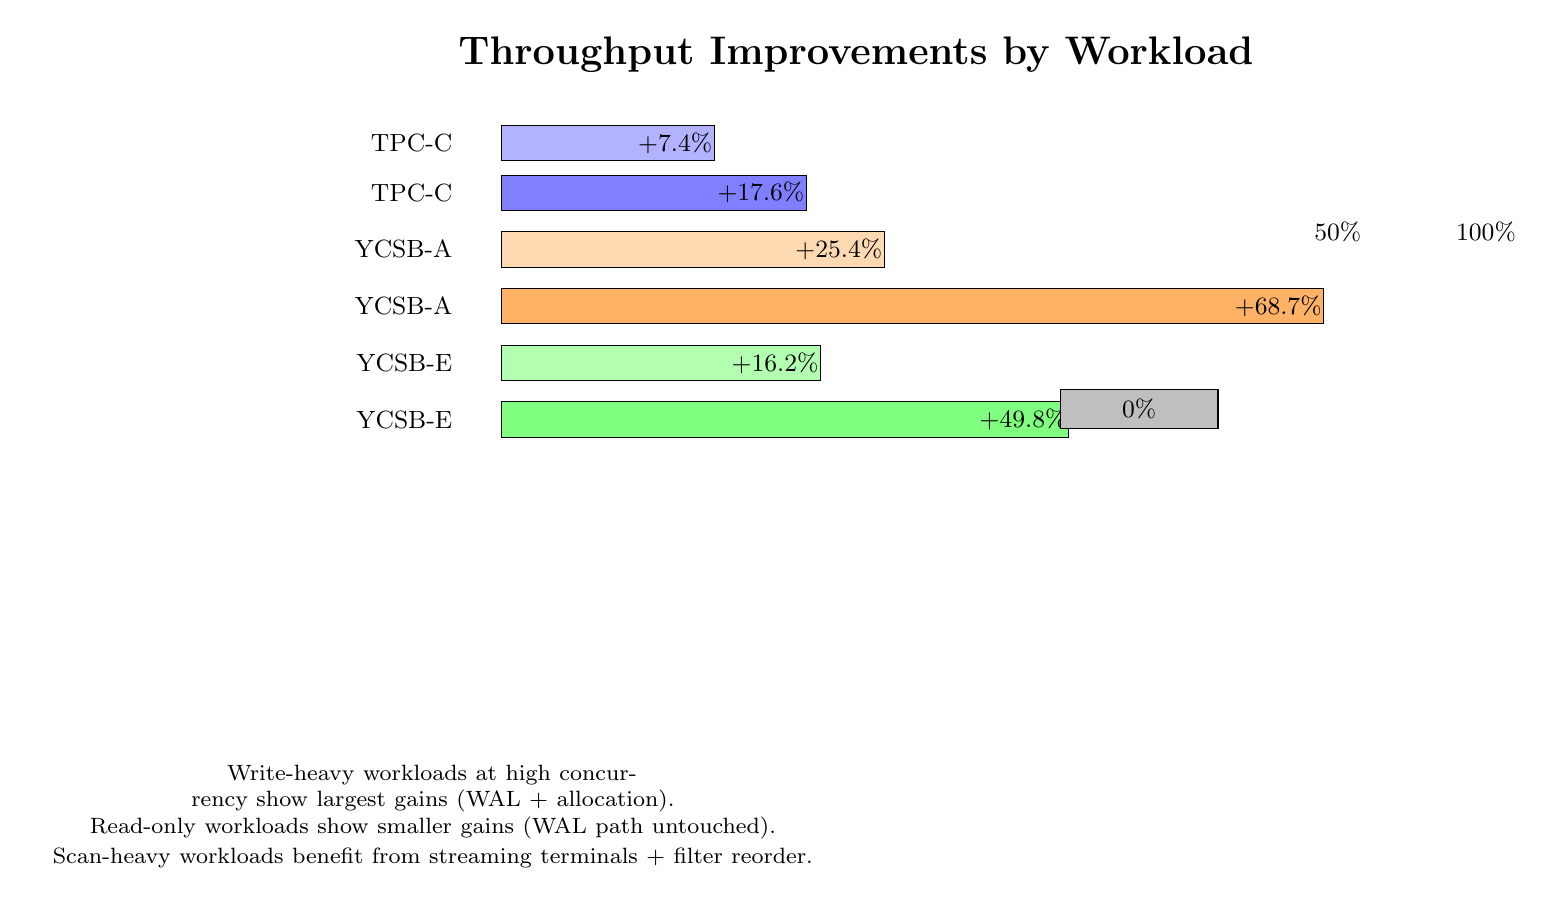
\begin{tikzpicture}[scale=0.9, every node/.style={font=\small}]
  % Title
  \node[font=\bfseries\Large] at (6, 9) {Throughput Improvements by Workload};

  % TPC-C @ 16 threads
  \draw[fill=blue!30] (1, 7.5) rectangle (4, 8);
  \node[left, xshift=-0.5cm] at (1, 7.75) {TPC-C};
  \node[left, xshift=0.1cm] at (4, 7.75) {\small +7.4\%};

  % TPC-C @ 64 threads
  \draw[fill=blue!50] (1, 6.8) rectangle (5.3, 7.3);
  \node[left, xshift=-0.5cm] at (1, 7.05) {TPC-C};
  \node[left, xshift=0.1cm] at (5.3, 7.05) {\small +17.6\%};

  % YCSB-A @ 16 threads
  \draw[fill=orange!30] (1, 6.0) rectangle (6.4, 6.5);
  \node[left, xshift=-0.5cm] at (1, 6.25) {YCSB-A};
  \node[left, xshift=0.1cm] at (6.4, 6.25) {\small +25.4\%};

  % YCSB-A @ 64 threads
  \draw[fill=orange!60] (1, 5.2) rectangle (12.6, 5.7);
  \node[left, xshift=-0.5cm] at (1, 5.45) {YCSB-A};
  \node[left, xshift=0.1cm] at (12.6, 5.45) {\small +68.7\%};

  % YCSB-E @ 16 threads
  \draw[fill=green!30] (1, 4.4) rectangle (5.5, 4.9);
  \node[left, xshift=-0.5cm] at (1, 4.65) {YCSB-E};
  \node[left, xshift=0.1cm] at (5.5, 4.65) {\small +16.2\%};

  % YCSB-E @ 64 threads
  \draw[fill=green!50] (1, 3.6) rectangle (9.0, 4.1);
  \node[left, xshift=-0.5cm] at (1, 3.85) {YCSB-E};
  \node[left, xshift=0.1cm] at (9.0, 3.85) {\small +49.8\%};

  % Legend
  \node[below, text width=10cm, text centered, yshift=-0.8cm] {
    \footnotesize Write-heavy workloads at high concurrency show largest gains (WAL + allocation). \\
    Read-only workloads show smaller gains (WAL path untouched). \\
    Scan-heavy workloads benefit from streaming terminals + filter reorder.
  };

  % Scale reference
  \node[draw, rectangle, fill=lightgray, minimum width=2cm, minimum height=0.3cm, below=2cm] at (10, 6.5) {\small 0\%};
  \node[right=0.3cm] at (12, 6.5) {50\%};
  \node[right=0.3cm] at (14, 6.5) {100\%};
\end{tikzpicture}
\caption{Combined throughput improvement from all optimizations across representative
workloads. Gains are highest in write-heavy, high-concurrency scenarios where WAL contention
and allocator pressure dominate baseline cost.}
\label{fig:combined_impact}
\end{figure}

\subsection{Optimization Categories}

\begin{figure}[h]
\centering
\begin{tikzpicture}[scale=0.85, every node/.style={font=\small}]
  % Title
  \node[font=\bfseries\Large] at (6, 10) {21 Optimizations by Category};

  % WAL optimizations
  \node[draw, rectangle, fill=red!20, rounded corners, minimum width=3cm, minimum height=3cm, align=center] (wal) at (2, 7) {
    \textbf{WAL \& Visibility} \\
    \small(5 opts) \\
    \\
    \tiny Native code gen \\
    CRC32 table \\
    Sharding \\
    Tickets \\
    Buffers
  };

  % Range scans
  \node[draw, rectangle, fill=orange!20, rounded corners, minimum width=3cm, minimum height=3cm, align=center] (scans) at (6, 7) {
    \textbf{Range Scans} \\
    \small(4 opts) \\
    \\
    \tiny Filter reorder \\
    Dyn removal \\
    Full-domain \\
    Streaming
  };

  % Transaction state
  \node[draw, rectangle, fill=yellow!20, rounded corners, minimum width=3cm, minimum height=3cm, align=center] (tx) at (10, 7) {
    \textbf{Transactions} \\
    \small(4 opts) \\
    \\
    \tiny Inline write set \\
    Reverse abort \\
    Read-only \\
    Cursor routing
  };

  % GC and sizing
  \node[draw, rectangle, fill=green!20, rounded corners, minimum width=3cm, minimum height=2cm, align=center] (gc) at (2, 2.5) {
    \textbf{GC \& Alloc} \\
    \small(3 opts) \\
    \tiny Sharding, reuse \\
    In-place, sizing
  };

  % Workload harness
  \node[draw, rectangle, fill=blue!20, rounded corners, minimum width=3cm, minimum height=2cm, align=center] (work) at (6, 2.5) {
    \textbf{Workload} \\
    \small(5 opts) \\
    \tiny Patch, hit/miss \\
    Zipf, sampling, modes
  };

  % Datastructure changes
  \node[draw, rectangle, fill=purple!20, rounded corners, minimum width=3cm, minimum height=2cm, align=center] (dstruct) at (10, 2.5) {
    \textbf{Datastructure} \\
    \small(6 changes) \\
    \tiny Split, masks \\
    Sizing, indirection
  };

  % Impact arrows
  \draw[->, thick, color=darkred] (wal.south) -- (3, 5.5);
  \node[left, font=\small\color{darkred}] at (2, 5.3) {68\% peak};

  \draw[->, thick, color=darkorange] (scans.south) -- (6, 5.5);
  \node[above, font=\small\color{darkorange}] at (6, 5.3) {+17\%};

  \draw[->, thick, color=darkgreen] (gc.north) -- (2, 4.5);
  \node[right, font=\small\color{darkgreen}] at (2.5, 4.3) {allocator};
\end{tikzpicture}
\caption{Optimization taxonomy: 6 datastructure changes plus 21 optimizations across 5
categories. WAL optimizations have the largest single impact on write-heavy workloads.}
\label{fig:optimization_categories}
\end{figure}

\subsection{Adoption Summary}

\begin{table}[h]
\centering
\small
\begin{tabular}{lll}
\toprule
\textbf{Optimization} & \textbf{Decision} & \textbf{Key Metric} \\
\midrule
1. Target-CPU Native & Adopted & Prerequisite \\
2. Table-Driven CRC32 & Adopted & +22.6\% $\to$ 11.3\% CPU (self-time) \\
3. Sharded WAL Channels & Adopted & 7.9\% $\to$ 0.3\% CPU (send) \\
4. Flush Ticket Removal & Adopted & +79\% synthetic throughput \\
5. Payload-Size Hints & Adopted & 7.1\% $\to$ 3.0\% allocator CPU \\
6. Filter Reorder & Adopted & +11\%--18\% narrow-scan latency \\
7. Remove Visibility Indirection & Adopted & Inlining improvement \\
8. Full-Domain Specialization & Adopted & Redundant-comparison removal \\
9. Zero-Copy Streaming & Adopted & +16.8\% full-scan throughput \\
10. Ordered Cursor Routing & Adopted & Correct, allocation-free \\
11. Inline Write Set & Adopted & Zero heap allocation (up to 16 keys) \\
12. Reverse-Order Abort & Adopted & Correctness requirement \\
13. Empty Read-Only Elision & Adopted & Clock/commit-log saving \\
14. Sharded Reuse Pool & Adopted & Allocator contention reduction \\
15. Update-In-Place & Adopted (conditional) & GC-dependent \\
16. Big-Tree Leaf Sizes & Adopted (Medium default) & Flat throughput, configurable \\
17. YCSB Single-Field Patch & Adopted & +90.8\% single-field updates \\
18. Point-Hit-Miss Only & Adopted & +2.07$\times$ read-only throughput \\
19. Walker-Alias Zipf & Adopted & $O(1)$ sampling \\
20. Amortized Sampling & Adopted & Measurement overhead reduction \\
21. YCSB Execution Modes & Adopted & Transparent comparison \\
\bottomrule
\end{tabular}
\caption{Optimization summary: all optimizations were adopted, some conditionally
or with specific configuration flags.}
\label{tab:opt_summary}
\end{table}

\subsection{Combined Performance Impact}

The cumulative effect of the datastructure changes and optimizations above produces:

\begin{table}[h]
\centering
\small
\begin{tabular}{lrrr}
\toprule
\textbf{Workload} & \textbf{Threads} & \textbf{Before Series} & \textbf{After Optimizations} \\
\midrule
TPC-C & 16 & 40,902 & 43,913 \\
TPC-C & 64 & 57,667 & 67,812 \\
YCSB-A (50\% update) & 16 & 1,603,135 & 2,010,940 \\
YCSB-A & 64 & 1,339,295 & 2,258,954 \\
YCSB-E (scan-heavy) & 16 & 2,137,315 & 2,483,067 \\
YCSB-E & 64 & 1,789,143 & 2,679,747 \\
\bottomrule
\end{tabular}
\caption{Combined throughput improvements from the full optimization series. Multiple
optimizations (WAL, visibility, allocation) contributed to each workload.}
\label{tab:combined_impact}
\end{table}

The most dramatic improvements appear in write-heavy workloads at high concurrency,
where WAL contention and allocator pressure are highest.

\subsection{Design Principles}

Throughout the optimization process, several recurring principles emerged:

\begin{enumerate}
  \item \textbf{Measure in context:} Isolated microbenchmarks motivated optimizations,
        but final decisions were based on end-to-end transaction throughput.

  \item \textbf{Share contention points carefully:} Sharding (WAL, reuse pools) was
        more effective than a single global lock, but too many shards adds memory overhead.

  \item \textbf{Move work off the hot path:} Setup-phase work (Zipf table construction,
        CRC32 table) is cheap compared to per-operation work.

  \item \textbf{Preserve allocation-free fast paths:} Inline structures (\code{SmallVec},
        inline arrays) enable common cases to avoid the heap.

  \item \textbf{Let the compiler specialize:} Removing indirection (\code{dyn} closures,
        type erasure) allows monomorphization and inlining.

  \item \textbf{Be explicit about configuration:} Modes (\code{atomic} vs. \code{transaction},
        \code{writeallfields}, leaf sizes) allow side-by-side comparison without changing
        underlying code.
\end{enumerate}

\newpage

\section{Open Issues and Future Work}
\label{sec:open}

Several issues remain open:

\begin{itemize}
  \item \textbf{TPC-C conflict rate at high contention:} At 8 warehouses and 64 terminals,
        Payment transactions experience $\sim$71--76\% conflict rates, and New-Order $\sim$47\%.
        This is pure wasted work on the write path and is unrelated to the WAL or allocation
        optimizations addressed in this document.

  \item \textbf{OLC backoff overhead:} Optimistic lock coupling's \code{\_\_sched\_yield}
        on retry accounts for $\sim$8--9\% of CPU cycles on contended writes. A smarter
        backoff strategy (adaptive delays, spinning) may improve this.

  \item \textbf{WAL buffer pooling:} Per-write allocations in \code{WalWriter} (fixed via
        Optimization~\ref{sec:wal_buffer_size}) could be further eliminated by reusing a
        bounded pool of buffers. The challenge is thread-safe ownership across channel
        handoff to the flush thread.

  \item \textbf{OLAP scan garbage tolerance:} Larger leaves (Huge) slow down aged OLAP scans
        because they retain more dead versions. A more aggressive per-table compaction or
        a separate OLAP-optimized leaf layout might help.

  \item \textbf{GC memory overhead:} The snapshot cache and worker structures grow with the
        configured thread budget, not the actual thread count. This is intentional (process-lifetime
        configuration) but can be wasteful in under-subscribed scenarios.
\end{itemize}

\newpage

\section{Conclusion}

The cMVBT-OSIC system demonstrates that a cache-conscious multiversion B-tree with
careful attention to allocation, contention, and compilation can achieve competitive
transaction throughput. The combination of datastructure changes (split leaf layout,
inline masks, exact page sizing) and targeted optimizations (WAL sharding, zero-copy
streaming, visibility caching) removed major CPU hotspots and allocator pressure points,
yielding improvements of 7--70\% across diverse workloads.

The design is not fundamentally novel: each individual optimization is a known technique
(split arrays, sharding, inlining closures). The contribution is in their careful
application to a snapshot-isolated, copy-on-write multiversion tree, demonstrating that
such a design need not sacrifice performance for correctness or ease of implementation.

\end{document}
